%!TEX root = ../../main.tex

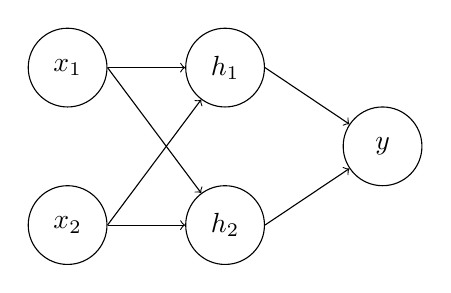
\begin{tikzpicture}
    \tikzstyle{node}=[circle, draw, minimum size=1cm];

    \node (x1) at (0, 2) [node] {$x_1$};
    \node (x2) at (0, 0) [node] {$x_2$};

    \node (h1) at (2, 2) [node] {$h_1$};
    \node (h2) at (2, 0) [node] {$h_2$};
    
    \node (y) at (4, 1) [node] {$y$};

    \draw (x1.east) edge[->] (h1);
    \draw (x1.east) edge[->] (h2);

    \draw (x2.east) edge[->] (h1);
    \draw (x2.east) edge[->] (h2);
    
    \draw (h1.east) edge[->] (y);
    \draw (h2.east) edge[->] (y);


\end{tikzpicture}